\graphicspath{
    {figures_and_references/urban_surface_detection/}
    {figures_and_references/EELISA_conference/}
}

% \selectlanguage{english}
\renewcommand{\chapternametext}{Chapter \thechapter: The \texttt{GeoImageVision} Python Package}

\begin{refsection}

\chapter{\chapternametext}
\

\renewcommand{\headingtextL}{}
\renewcommand{\headingtextR}{\chapternametext}
\begingroup
 \flushbottom
 \setlength{\parskip}{0pt plus 1fil}%
 \localtableofcontents 
\endgroup

\begingroup
 \flushbottom
 \setlength{\parskip}{0pt plus 1fil}%
 \locallistoffigures
\endgroup


\newpage

\setcounter{section}{0} 



\FloatBarrier

\renewcommand{\sectionnametext}{Automatic creation of aerial imagery datasets}
\renewcommand{\headingtextL}{\chapternametext}
\renewcommand{\headingtextR}{\thesection. \sectionnametext}
\section{\sectionnametext}

\subsection{Introduction}

Aerial imagery can be accessed through Open Geospatial Consortium service standards, such as WMS, WMTS or XYZ, usually used by government agencies and most aerial imagery providers like Google, ESA or NASA.


Ground truth data must be represented as vector data, typically in the form of polygons that delineate the objects targeted for segmentation.  Utilizing vector data ensures seamless compatibility across various coordinate systems and resolutions.  Maintaining a consistent coordinate system throughout the workflow is crucial, converting both the image grid and the ground truth data to the same coordinate system. Raster ground truth data can be transformed into vector format using tools like rasterio \footcite{gillies_rasterio_2013}. 


The \texttt{GeoVisionDataset} Python package \footcite{urena_pliego_transport-related_2025} was specifically developed to streamline this process. It enables efficient creation of machine learning-ready datasets using open-access geospatial data. Key features of the package include:

\begin{itemize}
    \item Automatic generation of spatial grids over a defined region.
    \item Support for downloading imagery from Open Geospatial Consortium (OGC) providers such as WMS, WMTS, and XYZ, commonly used by governmental agencies.
    \item Integration sources like Google Satellite imagery and other widely used providers.
    \item Ground truth data acquisition in both vector and raster formats, either via standard OGC protocols such as WFS or through the OpenStreetMap database using Overpass Turbo API queries.
    \item Automatic handling of ground truth and aerial imagery coordinate systems.
    \item Download of dataset ground truth and images in common machine learning formats such as COCO. 
\end{itemize}

With the \textit{GeoVisionDataset} package multiple datasets were created for the experiments in this study: a separate dataset for each of the three study areas was generated, where automatic footprint extraction models were trained, as well as a dataset for Madrid and Vienna focused on segmenting transportation-related surfaces.



\subsection{Dataset grid}

Transformer-based models typically require input images of fixed pixel dimensions, whereas convolutional neural networks (CNNs) can process images of varying sizes. Nevertheless, it is generally recommended that all images within a dataset have similar spatial dimensions and resolutions in both cases. This consistency helps preserve the visual characteristics of features in the images, ensuring that the data used during inference closely resembles the data seen during training.

To construct a dataset, one or more polygons are designated as the region of interest. A grid structure is then generated over this area to facilitate the download of aerial imagery and corresponding ground truth data in formats suitable for training machine learning models (fig. \ref{fig:grid}).
\begin{figure}[!htp]
    \centering
    \begin{tabular}{cc}
        \begin{subfigure}[t]{0.47\linewidth}
            \centering
            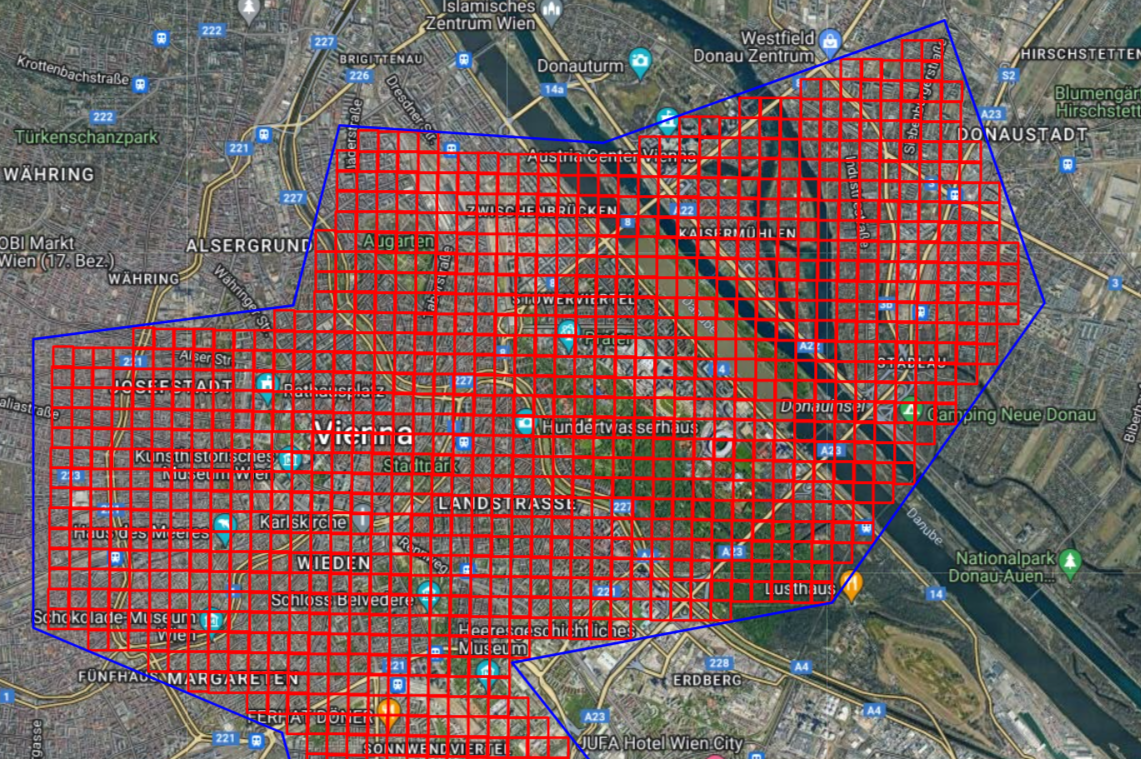
\includegraphics[width=6cm, height=3.5cm]{figures/fig_grid_global.png}
            \caption{Dataset region (blue) and generated dataset grid (red).}
            \label{fig:grid_exaple}
        \end{subfigure} &
        \begin{subfigure}[t]{0.47\linewidth}
            \centering
            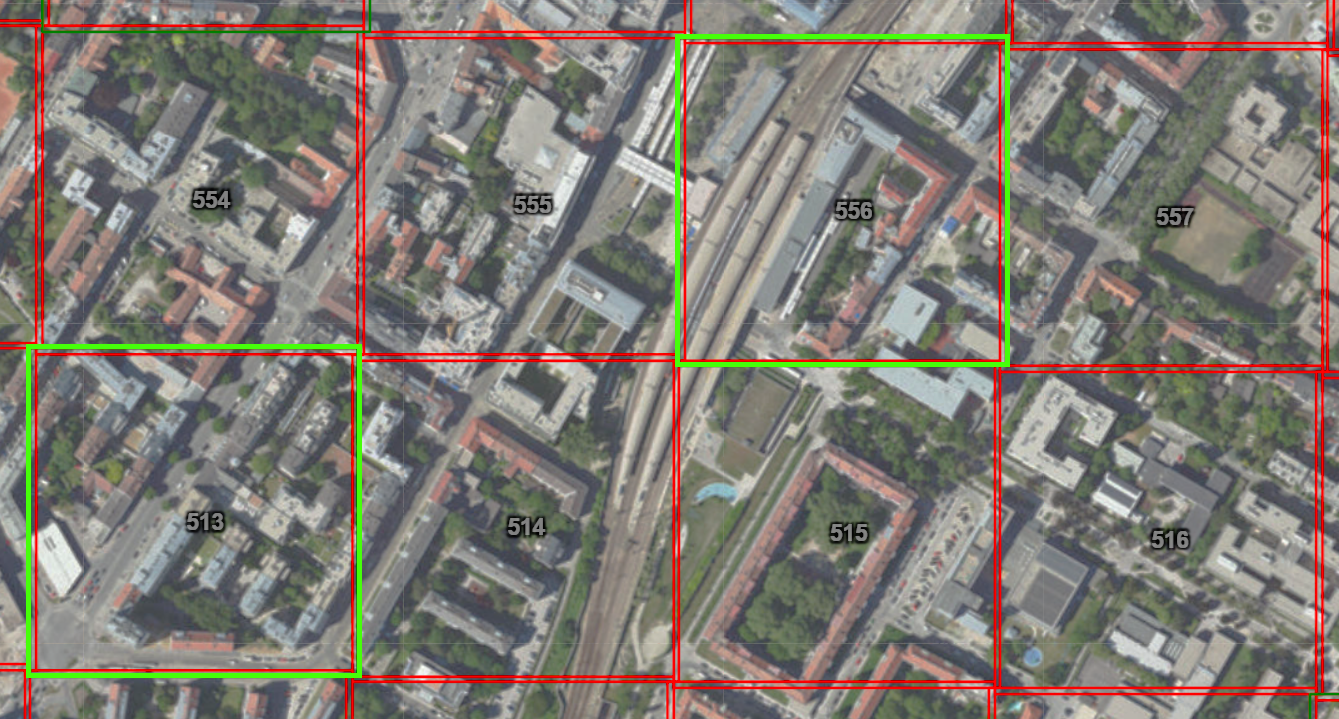
\includegraphics[width=6cm, height=3.5cm]{figures/fig_grid_local.png}
            \caption{Detail of the tiles in the grid. In green tiles randomly selected for the dataset. Numbers are the tile ids. Overlap is set to 0 m.}
            \label{fig:grid_detail}
        \end{subfigure}
    \end{tabular}
    \caption{Dataset grid example.}
    \label{fig:grid}
\end{figure}

The procedure involves defining a grid in UTM coordinates, shaped as a rectangle,
based on the overall bounds of the dataset region. This grid is established with
a specified tile size and overlap between tiles. As minimum and maximum values for x and y coordinates are needed to georeference a matrix and save it as a image, tiles are defined as minimum and maximum x and y values. After forming the grid, all coordinates are
converted to the coordinate system of the image provider. This conversion might
adjust the grid bounds, as they could appear rotated. The reason for this is that the x and y axis can rotate during the coordinate conversion and, to cover the minimum and maximum x and y values from the previous coordinate system a larger area has to be selected and tiles can overlap slightly. In figure \ref{fig:grid} tiles exhibit this situation due to the aerial image being in geographic coordinates
while the grid is in UTM resulting in a small misalignment and overlap of the tile bounds. The grid is then converted to the coordinates of the
image to accurately preserve the image bounds. Similarly, the mask in vector
format undergoes conversion to the image's coordinate system. Incorporating
overlap between tiles could be important for precise results at the image borders,
helping prevent errors caused by partially visible objects. The overlap can
also be configured accordingly. 

\subsection{Ground truth}

Ground truth data must be in the form of vector data, represented as polygons that delineate the objects targeted for segmentation. The use of vector data allows for seamless compatibility with various coordinate systems and resolutions. It is crucial to maintain the coordinate system used by the image provider consistently, necessitating the conversion of both the grid and ground truth to the coordinate system of the images. If the ground truth is initially presented as raster data, it can be transformed into vector data using tools such as rasterio \footcite{gillies_rasterio_2013}. \\


A challenge arises when cartography is available as line data instead of polygons. 
Consequently, polygons need to be generated by connecting the lines that enclose 
the desired objects. This adds inaccuracies in the data. 

\renewcommand{\sectionnametext}{Foundational image vision models}
\renewcommand{\headingtextR}{\thesection. \sectionnametext}
\section{\sectionnametext}

\subsection{Semantic segmentation models}
This paper aims to develop a practical machine learning vision workflow that delivers high-quality results without requiring training on a large compute cluster. The approach developed in this paper is to fine-tune a pre-trained foundational model using a task-specific dataset. Among the top-performing models currently available is the SAM model \footcite{kirillov_segment_2023}.
The pre-trained image encoder of the SAM model 
was employed, with only a new convolutional decoder being trained in
accordance with a U-Net like structure (fig. \ref{fig:transformer}). The convolutional decoder consists of four layers with channel depths of 256, 128, 64, and 32, respectively. It is integrated with a pre-trained image encoder from the SAM base model, which also has a depth of four. To enhance feature integration, four skip connections link corresponding layers of the image encoder and the decoder. The image encoder is a vision transformer, with its weights initialized using the publicly available checkpoint vit-b from a model trained with masked autoencoders on the SA-1B dataset \footcite{he_masked_2022, kirillov_segment_2023}, specifically for images with a resolution of 1024x1024 pixels. 
The implementation utilizes the pytorch-lightning \footcite{falcon_pytorch_2023}
and segmentation models \footcite{iakubovskii_segmentation_models_pytorch_2019}
Python libraries. \\

\begin{figure}[!htp]
    
    \centering
    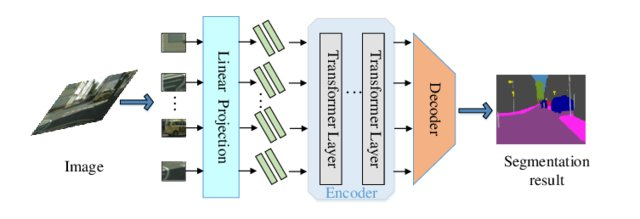
\includegraphics[width=9cm]{figures/fig_transformer_model.jpg}
    
    \caption{Transformer-based model (Source: Dosovitskiy et al., 2020)}
    \label{fig:transformer}
\end{figure} 

Loss functions for semantic segmentation tasks can be categorized into pixel,
boundary, and region-level loss functions \footcite{azad_loss_2023}. In the case of training datasets featuring unbalanced classes, such as in this study, where smaller surfaces are detected over a main background class, the asymmetrical unified focal loss function \footcite{yeung_unified_2022} is an adecuate loss function for model training. This combined loss  integrates the Tversky loss (region loss) with the focal loss (pixel loss) function. \\


The diversity of the images was measured calculating the dot product 
of the class count vector (number of pixels of each class in the image) of each image respect to the median value of the dataset. Images with lower diversity values are repeated more often during the training process.  


\subsection{Instance segmentation}


Two types of assistant models are proposed for instance segmentation tasks such as building footprint extraction \footcite{osco_segment_2023}:

\begin{itemize}
    \item Fully Automated Segmentation: An instance segmentation model is used to automatically generate the building footprint geometry for all visible structures in an image (zero-shot segmentation). Although this method does not require user input during segmentation, results may not be fully accurate in all cases, and post-review by the user is necessary.

    \item Assisted Segmentation: The user selects a point inside the building to be segmented, and the model returns the footprint geometry automatically (one-shot segmentation). This approach is more accurate due to the additional user input and ensures that all results are reviewed by the user.
\end{itemize}

For fully automated segmentation the Mask2Former \footcite{cheng_masked-attention_2022} is fine tuned and trained with the datasets created in the 3 strudy areas dividing the tiles into training and validation.


For assisted automated segmentation the SAM2 model \footcite{ravi_sam_2024} is fine tuned and trained with the same datasets, training and testing tiles.

\newpage

\renewcommand{\sectionnametext}{References}
\renewcommand{\headingtextR}{\thesection. \sectionnametext}
\section{\sectionnametext}

\printbibliography[heading=none]


\end{refsection}